\documentclass[../main.tex]{subfiles}
\begin{document}

\section{Desarrollo}\label{sec:desarrollo}

Para tener un aislamiento de recursos se utiliza \href{https://www.docker.com/}{docker} y así tener un entorno limpio
de trabajo para poder analizar de mejor manera los resultados de cada prueba.

\subsection{Test de algoritmos criptográficos}\label{test-de-algoritmos-criptograficos}

\subsubsection{Instrucciones de uso}\label{instrucciones-de-uso}

Hay que tener \texttt{docker} y \texttt{docker-compose} instalado

Se corre el siguiente comando la primera vez que se utiliza

\begin{code}
\begin{minted}{shell-session}
$ docker-compose build
\end{minted}
\end{code}
Se corre el siguiente comando cada que se quiera ejecutar
\begin{code}
\begin{minted}{shell-session}
$ docker-compose up
\end{minted}
\end{code}
Los resultados de la ejecución se encontrarán en el directorio \texttt{./results/}
(tomando la raíz del proyecto):

\subsection{Operaciones y probar}\label{clasificaciuxf2n-de-operaciones}
\subsubsection{Cifrado y descifrado}\label{sec:cifrado-y-descifrado}
En esta clasificación se encuentran:
\begin{itemize}
  \item AES-EBC 256 bits
  \item AES-CBC 256 bits
  \item RSA-OAEP\footnote{Este ultimo no es comparable con AES-EBC y CBC} 1024 bits
\end{itemize}
Se usan bibliotecas ya escritas para ejecutar las pruebas:
\begin{code}
  \caption{Código que ejecuta las pruebas de AES}\label{sec:cifrado-y-descifrado-1}
  \inputminted[lastline=81]{python}{../src/test_algoritmos_crypto/AESTests.py}
\end{code}

\textit{RSA\_OAEP} también se usa para firmar, verificar, cifrar y verificar.
\begin{code}
  \caption{Código que ejecuta las pruebas de RSA\_OAEP}\label{sec:cifrado-y-descifrado-2}
  \inputminted[lastline=65]{python}{../src/test_algoritmos_crypto/RSAOAEPTest.py}
\end{code}

\subsubsection{Hashing}\label{hashing}
En esta clasificación se encuentra:
\begin{itemize}
  \item SHA-2 384 bits
  \item SHA-2 512 bits
  \item SHA-3 512 bits
\end{itemize}
\begin{code}
  \caption{Código que ejecuta las pruebas SHA2 y SHA3}\label{sec:hashing}
  \inputminted[lastline=56]{python}{../src/test_algoritmos_crypto/SHATests.py}
\end{code}

\subsubsection{Firma y verificación}\label{firma-y-verificacion}
Aquí se encuentran:
\begin{itemize}
  \item RSA-PSS 1024 bits
  \item DSA 1024 bits
  \item ECDSA Prime Field 521 bits
  \item ECDSA Binary Field 571 bits
\end{itemize}
\begin{code}
  \caption{Código que ejecuta las pruebas firma y verificación}\label{sec:firma-y-verificacion-1}
  \inputminted[lastline=149]{python}{../src/test_algoritmos_crypto/SignVerifTests.py}
\end{code}

\newpage{}

\subsubsection{Resultados}\label{sec:resultados}

En esta sección mostramos los resultados generados.

\paragraph{Cifrado y descifrado}\label{sec:aes_res}
En la siguiente tabla~\ref{tab:aes} se comparan los algoritmos de AES, el AES-CBC vs AES-ECB, ambos realizando
el cifrado y el descifrado (tomando el tiempo como segundos $[s]$).
\begin{table}[H]
  \centering
  \caption{Resultados AES}\label{tab:aes}
  \begin{tabular}{|c|c|c|c|c|}
    \hline
    \rowcolor[HTML]{000000}
    {\color[HTML]{FFFFFF} Nombre} & \multicolumn{1}{l|}{\cellcolor[HTML]{000000}{\color[HTML]{FFFFFF} aes-cbc-encrypt}} & \multicolumn{1}{l|}{\cellcolor[HTML]{000000}{\color[HTML]{FFFFFF} aes-cbc-decrypt}} & \multicolumn{1}{l|}{\cellcolor[HTML]{000000}{\color[HTML]{FFFFFF} aes-ecb-encrypt}} & \multicolumn{1}{l|}{\cellcolor[HTML]{000000}{\color[HTML]{FFFFFF} aes-ecb-decrypt}} \\ \hline
    014730f80ac625fe84f026c60bfd547d & $\num{846.19E-06}$ & $\num{89.53E-06}$ & $\num{291.35E-06}$ & $\num{65.76E-06}$ \\ \hline
    \rowcolor[HTML]{C0C0C0}
    0b24af36193ce4665f2825d7b4749c98 & $\num{77.93E-06}$ & $\num{45.45E-06}$ & $\num{30.63E-06}$ & $\num{27.99E-06}$ \\ \hline
    761c1fe41a18acf20d241650611d90f1 & $\num{85.46E-06}$ & $\num{37.12E-06}$ & $\num{30.95E-06}$ & $\num{27.66E-06}$ \\ \hline
    \rowcolor[HTML]{C0C0C0}
    8a560769d605868ad80d819bdba03771 & $\num{104.16E-06}$ & $\num{56.96E-06}$ & $\num{36.18E-06}$ & $\num{30.09E-06}$ \\ \hline
    91fbef2d15a97816060bee1feaa49afe & $\num{95.12E-06}$ & $\num{40.32E-06}$ & $\num{35.50E-06}$ & $\num{30.57E-06}$ \\ \hline
    \rowcolor[HTML]{C0C0C0}
    pdf de prueba & $\num{257.92E-06}$ & $\num{175.73E-06}$ & $\num{83.41E-06}$ & $\num{50.42E-06}$ \\ \hline
    imagen de prueba & $\num{213.56E-06}$ & $\num{154.80E-06}$ & $\num{67.87E-06}$ & $\num{53.29E-06}$ \\ \hline
    \rowcolor[HTML]{C0C0C0}
    zip de prueba & $\num{9.73E-03}$ & $\num{8.26E-03}$ & $\num{4.75E-03}$ & $\num{2.04E-03}$ \\ \hline
  \end{tabular}
\end{table}

Gráficamente, en la figura~\ref{fig:aes}, se ve una clara ventaja del AES-ECB siendo más rápido que AES-CBC, sin embargo, el
AES-ECB es más susceptible de revelar patrones de texto que cualquier otro método (figura~\ref{fig:ejem}).

\begin{figure}
\begin{subfigure}[b]{0.55\textwidth}
  \centering
  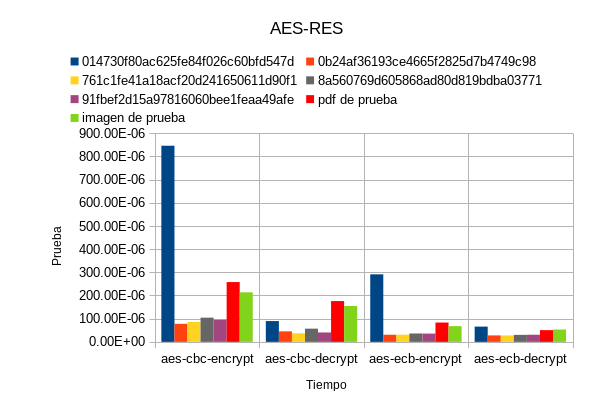
\includegraphics[width=\textwidth]{aes-res-res}
  \caption{Resultado AES}\label{fig:aes}
\end{subfigure}
\hfill{}
\begin{subfigure}[b]{0.4\textwidth}
  \centering
  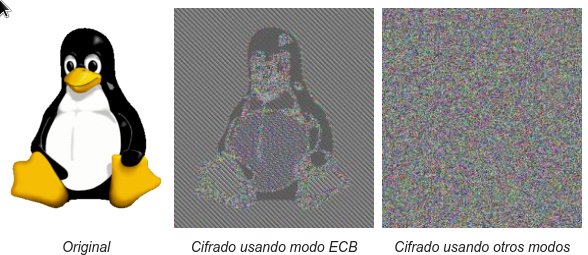
\includegraphics[width=\textwidth]{ecb}
  \caption{Versión de mapa de bits de una imagen cifrado de dos distintas maneras}\label{fig:ejem}
\end{subfigure}
% \caption{Resultados AES}
\end{figure}

\newpage{}


El modo ECB puede hacer que protocolos sin protección de integridad sean aún más
susceptibles a ataques de repetición, dado que cada bloque es descifrado de la misma
manera.

También se compara el algoritmo \textbf{RSA\_OAEP}, este también tiene los métodos
de cifrado y descifrado, sin embargo este es sumamente más lento a comparación
de las anteriores, \textbf{RSA\_OAEP} también sirve para firma y verificación
(apartado~\ref{sec:firma-y-verificacion}).
\begin{figure}[ht]
  \centering{}
  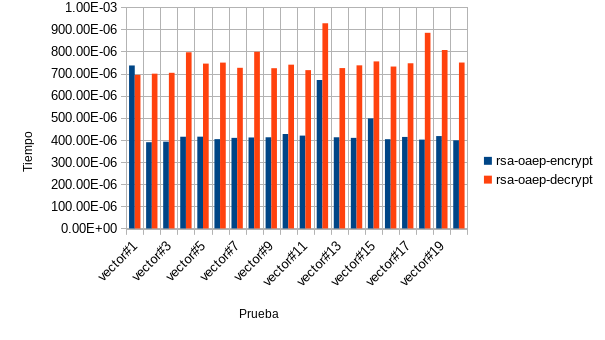
\includegraphics[width=0.6\textwidth]{rsa-oaep-res}
  \caption{Resultado RSA\_OAEP}\label{fig:rsa-oaep}
\end{figure}

\begin{table}[ht]
\centering{}
  \caption{Resultados RSA\_OAEP}\label{tab:rsa}
  \begin{tabular}{|c|c|c|}
    \rowcolor[HTML]{000000}
    {\color[HTML]{FFFFFF} nombre} & {\color[HTML]{FFFFFF} rsa-oaep-encrypt} & {\color[HTML]{FFFFFF} rsa-oaep-decrypt} \\
    vector\#1  & $\num{736.55E-06}$ & $\num{694.37E-06}$ \\ \hline
    \rowcolor[HTML]{C0C0C0}
    vector\#2  & $\num{389.95E-06}$ & $\num{699.84E-06}$ \\ \hline
    vector\#3  & $\num{392.42E-06}$ & $\num{703.46E-06}$ \\ \hline
    \rowcolor[HTML]{C0C0C0}
    vector\#4  & $\num{414.55E-06}$ & $\num{796.44E-06}$ \\ \hline
    vector\#5  & $\num{414.95E-06}$ & $\num{745.14E-06}$ \\ \hline
    \rowcolor[HTML]{C0C0C0}
    vector\#6  & $\num{403.66E-06}$ & $\num{749.80E-06}$ \\ \hline
    vector\#7  & $\num{409.28E-06}$ & $\num{726.27E-06}$ \\ \hline
    \rowcolor[HTML]{C0C0C0}
    vector\#8  & $\num{411.23E-06}$ & $\num{798.57E-06}$ \\ \hline
    vector\#9  & $\num{412.05E-06}$ & $\num{724.35E-06}$ \\ \hline
    \rowcolor[HTML]{C0C0C0}
    vector\#10 & $\num{426.96E-06}$ & $\num{740.39E-06}$ \\ \hline
    vector\#11 & $\num{419.66E-06}$ & $\num{715.59E-06}$ \\ \hline
    \rowcolor[HTML]{C0C0C0}
    vector\#12 & $\num{671.03E-06}$ & $\num{927.38E-06}$ \\ \hline
    vector\#13 & $\num{412.14E-06}$ & $\num{724.79E-06}$ \\ \hline
    \rowcolor[HTML]{C0C0C0}
    vector\#14 & $\num{409.40E-06}$ & $\num{737.38E-06}$ \\ \hline
    vector\#15 & $\num{497.37E-06}$ & $\num{755.24E-06}$ \\ \hline
    \rowcolor[HTML]{C0C0C0}
    vector\#16 & $\num{403.33E-06}$ & $\num{731.83E-06}$ \\ \hline
    vector\#17 & $\num{413.87E-06}$ & $\num{746.71E-06}$ \\ \hline
    \rowcolor[HTML]{C0C0C0}
    vector\#18 & $\num{401.73E-06}$ & $\num{884.51E-06}$ \\ \hline
    vector\#19 & $\num{417.54E-06}$ & $\num{806.70E-06}$ \\ \hline
    \rowcolor[HTML]{C0C0C0}
    vector\#20 & $\num{398.33E-06}$ & $\num{750.11E-06}$ \\ \hline
  \end{tabular}
\end{table}


\newpage{}

\subsubsection{Hashing}\label{sec:hash}

En este apartado comparamos sumas hash (tabla~\ref{tab:hash-res}), donde probamos con caracteres de diferente tamaño
y dos tipos de binarios distintos, como es esperado, las operaciones de 384 bits son más eficientes
que las operaciones de 512 bits. También es notoria la diferencia de tiempo de SHA-3 y SHA-2, siendo esta
última más veloz, sin embargo, el SHA-3 se puede implementar a través de hardware, por lo que
entonces el SHA-3 puede ser igual de rápido e incluso más rápido que el SHA-2

\begin{figure}[ht]
  \centering
  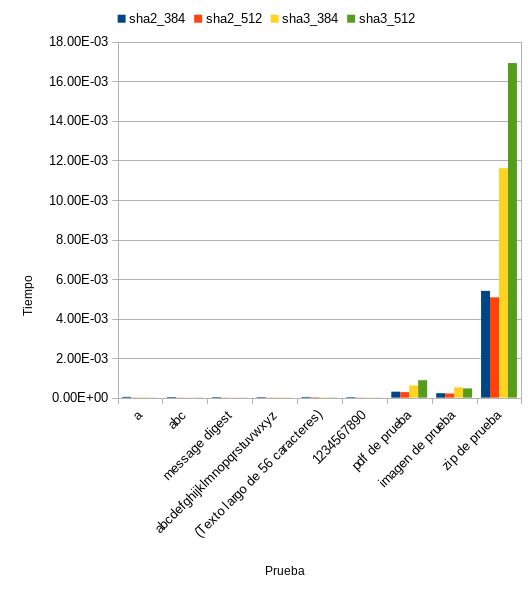
\includegraphics[width=0.4\textwidth]{hash_res}
  \caption{Resultado Hash}\label{fig:hash}
\end{figure}

\begin{table}[ht]
  \centering
  \caption{Resultados Hash}\label{tab:hash-res}
  \begin{tabular}{|c|c|c|c|c|}
    \hline
    \rowcolor[HTML]{000000}
    {\color[HTML]{FFFFFF} nombre} & {\color[HTML]{FFFFFF} sha2\_384} & {\color[HTML]{FFFFFF} sha2\_512} & {\color[HTML]{FFFFFF} sha3\_384} & {\color[HTML]{FFFFFF} sha3\_512} \\ \hline
    a                          & $\num{39.32E-06}$  & $\num{7.02E-06 }$  & $\num{19.27E-06}$  & $\num{4.97E-06}$   \\ \hline
    \rowcolor[HTML]{C0C0C0}
    abc                        & $\num{28.87E-06}$  & $\num{7.29E-06 }$  & $\num{13.19E-06}$  & $\num{6.22E-06}$   \\ \hline
    message digest             & $\num{27.01E-06}$  & $\num{6.66E-06 }$  & $\num{12.54E-06}$  & $\num{4.47E-06}$   \\ \hline
    \rowcolor[HTML]{C0C0C0}
    abcdefghijklmnopqrstuvwxyz & $\num{28.33E-06}$  & $\num{7.29E-06 }$  & $\num{13.74E-06}$  & $\num{5.64E-06}$   \\ \hline
    (Texto largo de 56 caracteres)              & $\num{35.41E-06}$  & $\num{20.68E-06}$  & $\num{18.56E-06}$  & $\num{6.91E-06}$   \\ \hline
    \rowcolor[HTML]{C0C0C0}
    1234567890                 & $\num{27.87E-06}$  & $\num{6.43E-06 }$  & $\num{11.80E-06}$  & $\num{4.58E-06}$   \\ \hline
    pdf de prueba              & $\num{300.25E-06}$ & $\num{276.33E-06}$ & $\num{619.34E-06}$ & $\num{882.02E-06}$ \\ \hline
    \rowcolor[HTML]{C0C0C0}
    imagen de prueba           & $\num{224.56E-06}$ & $\num{209.05E-06}$ & $\num{523.27E-06}$ & $\num{466.85E-06}$ \\ \hline
    zip de prueba              & $\num{5.40E-03 }$  & $\num{5.07E-03 }$  & $\num{11.61E-03}$  & $\num{16.93E-03}$  \\ \hline
  \end{tabular}
\end{table}


\newpage{}

\subsubsection{Firma y verificación}\label{sec:firma-y-verificacion}

Se comparó la eficiencia de firma y verificación de los algoritmos (tabla
~\ref{tab:hash-res}) \textbf{RSA\_PSS}, \textbf{DSA} y \textbf{ECDSA\_PRIME}. Entre todos
los algoritmos de firma y verificación esta claro que \textbf{DSA} es el más rápido de
todos para dichas tareas, sin embargo, como se mencionó anteriormente en el
apartado~\ref{sec:aes_res}, \textit{RSA} también sirve para cifrar y descifrar
simplemente invirtiendo el orden en el que se utilizan los exponentes.
\begin{table}[ht]
  \scriptsize
  \centering
  \caption{Resultados Firma y verificación}\label{tab:hash-res}
  \begin{tabular}{|c|c|c|c|c|c|c|c|c|}
    \hline
    \rowcolor[HTML]{000000}
    {\color[HTML]{FFFFFF} nombre} &
  {\color[HTML]{FFFFFF} ecdsa-binary-signing} &
  {\color[HTML]{FFFFFF} ecdsa-binary-verif} &
  {\color[HTML]{FFFFFF} ecdsa-prime-signing} &
  {\color[HTML]{FFFFFF} ecdsa-prime-verif} &
  {\color[HTML]{FFFFFF} dsa-signing} &
  {\color[HTML]{FFFFFF} dsa-verif} &
  {\color[HTML]{FFFFFF} rsa-pss-signing} &
  {\color[HTML]{FFFFFF} rsa-pss-verif} \\ \hline
    vector\#1  & $\num{2.59E-03}$ & $\num{4.64E-03}$ & $\num{4.07E-04}$ & $\num{7.80E-04}$ & $\num{5.22E-04}$ & $\num{2.95E-04}$ & $\num{9.19E-04}$ & $\num{2.70E-04}$ \\ \hline
    \rowcolor[HTML]{C0C0C0}
    vector\#2 & $\num{2.17E-03}$ & $\num{4.16E-03}$ & $\num{3.75E-04}$ & $\num{6.33E-04}$ & $\num{3.96E-04}$ & $\num{2.88E-04}$ & $\num{6.60E-04}$ & $\num{2.55E-04}$ \\ \hline
    vector\#3 & $\num{2.17E-03}$ & $\num{4.51E-03}$ & $\num{4.96E-04}$ & $\num{6.53E-04}$ & $\num{4.77E-04}$ & $\num{2.84E-04}$ & $\num{6.74E-04}$ & $\num{2.70 E-04}$ \\ \hline
    \rowcolor[HTML]{C0C0C0}
    vector\#4 & $\num{2.63E-03}$ & $\num{4.75E-03}$ & $\num{3.78E-04}$ & $\num{6.36E-04}$ & $\num{4.09E-04}$ & $\num{2.78E-04}$ & $\num{6.58E-04}$ & $\num{2.62E-04}$ \\ \hline
    vector\#5  & $\num{2.18E-03}$ & $\num{4.18E-03}$ & $\num{3.44E-04}$ & $\num{6.47E-04}$ & $\num{4.33E-04}$ & $\num{2.82E-04}$ & $\num{6.63E-04}$ & $\num{2.66E-04}$ \\ \hline
    \rowcolor[HTML]{C0C0C0}
    vector\#6  & $\num{2.25E-03}$ & $\num{4.34E-03}$ & $\num{3.98E-04}$ & $\num{6.48E-04}$ & $\num{4.00E-04}$ & $\num{2.92E-04}$ & $\num{6.72E-04}$ & $\num{2.59E-04}$ \\ \hline
    vector\#7  & $\num{2.20E-03}$ & $\num{4.28E-03}$ & $\num{3.66E-04}$ & $\num{6.44E-04}$ & $\num{3.93E-04}$ & $\num{2.86E-04}$ & $\num{8.12E-04}$ & $\num{3.35E-04}$ \\ \hline
    \rowcolor[HTML]{C0C0C0}
    vector\#8  & $\num{2.97E-03}$ & $\num{5.67E-03}$ & $\num{4.82E-04}$ & $\num{8.99E-04}$ & $\num{4.39E-04}$ & $\num{3.15E-04}$ & $\num{7.67E-04}$ & $\num{3.15E-04}$ \\ \hline
    vector\#9  & $\num{2.27E-03}$ & $\num{4.08E-03}$ & $\num{3.33E-04}$ & $\num{6.95E-04}$ & $\num{4.67E-04}$ & $\num{3.08E-04}$ & $\num{7.49E-04}$ & $\num{3.04E-04}$ \\ \hline
    \rowcolor[HTML]{C0C0C0}
    vector\#10 & $\num{2.52E-03}$ & $\num{5.25E-03}$ & $\num{4.94E-04}$ & $\num{1.28E-03}$ & $\num{4.23E-04}$ & $\num{2.89E-04}$ & $\num{6.93E-04}$ & $\num{2.81E-04}$ \\ \hline
    vector\#11 & $\num{2.24E-03}$ & $\num{4.33E-03}$ & $\num{3.98E-04}$ & $\num{6.49E-04}$ & $\num{4.23E-04}$ & $\num{3.05E-04}$ & $\num{6.82E-04}$ & $\num{2.76E-04}$ \\ \hline
    \rowcolor[HTML]{C0C0C0}
    vector\#12 & $\num{2.31E-03}$ & $\num{4.25E-03}$ & $\num{3.48E-04}$ & $\num{6.51E-04}$ & $\num{3.96E-04}$ & $\num{2.90E-04}$ & $\num{6.60E-04}$ & $\num{2.83E-04}$ \\ \hline
    vector\#13 & $\num{2.42E-03}$ & $\num{4.81E-03}$ & $\num{4.41E-04}$ & $\num{6.88E-04}$ & $\num{5.66E-04}$ & $\num{2.92E-04}$ & $\num{6.82E-04}$ & $\num{2.91E-04}$ \\ \hline
    \rowcolor[HTML]{C0C0C0}
    vector\#14 & $\num{2.33E-03}$ & $\num{4.57E-03}$ & $\num{3.79E-04}$ & $\num{6.79E-04}$ & $\num{4.50E-04}$ & $\num{2.98E-04}$ & $\num{6.76E-04}$ & $\num{2.68E-04}$ \\ \hline
    vector\#15 & $\num{2.29E-03}$ & $\num{4.31E-03}$ & $\num{3.58E-04}$ & $\num{6.75E-04}$ & $\num{3.93E-04}$ & $\num{2.84E-04}$ & $\num{7.83E-04}$ & $\num{2.92E-04}$ \\ \hline
    \rowcolor[HTML]{C0C0C0}
    vector\#16 & $\num{2.26E-03}$ & $\num{4.31E-03}$ & $\num{3.54E-04}$ & $\num{7.35E-04}$ & $\num{4.19E-04}$ & $\num{2.89E-04}$ & $\num{6.83E-04}$ & $\num{2.78E-04}$ \\ \hline
    vector\#17 & $\num{2.26E-03}$ & $\num{4.87E-03}$ & $\num{4.05E-04}$ & $\num{6.67E-04}$ & $\num{3.89E-04}$ & $\num{2.91E-04}$ & $\num{6.94E-04}$ & $\num{2.80E-04}$ \\ \hline
    \rowcolor[HTML]{C0C0C0}
    vector\#18 & $\num{2.40E-03}$ & $\num{4.43E-03}$ & $\num{3.58E-04}$ & $\num{6.68E-04}$ & $\num{4.16E-04}$ & $\num{2.84E-04}$ & $\num{6.90E-04}$ & $\num{2.77E-04}$ \\ \hline
    vector\#19 & $\num{2.30E-03}$ & $\num{4.39E-03}$ & $\num{3.60E-04}$ & $\num{6.75E-04}$ & $\num{4.31E-04}$ & $\num{2.95E-04}$ & $\num{6.67E-04}$ & $\num{2.70E-04}$ \\ \hline
    \rowcolor[HTML]{C0C0C0}
    vector\#20 & $\num{2.26E-03}$ & $\num{4.99E-03}$ & $\num{4.13E-04}$ & $\num{6.78E-04}$ & $\num{3.99E-04}$ & $\num{2.93E-04}$ & $\num{6.97E-04}$ & $\num{2.74E-04}$ \\ \hline
  \end{tabular}
\end{table}

Comparando \textit{RSA} con \textit{ECDSA} (se aprecia mejor en la figura~\ref{fig:fyv}),
esta última es más lenta (para niveles de seguridad más altos), no obstante esto no
significa que \textit{RSA} sea malo, las firmas \textit{ECDSA} como las claves públicas
son mucho más pequeñas que las firmas \textit{RSA} y las claves públicas de niveles de
seguridad similares. Si compara una curva \textit{ECDSA} de 192 bits con una clave RSA de
1k (que tienen aproximadamente el mismo nivel de seguridad; la curva \textit{ECDSA} de
192 bits es probablemente un poco más fuerte); luego, la firma \textit{RSA} y la clave
pública se pueden expresar en 128 bytes cada una (suponiendo que esté dispuesto a usar un
formato que ahorre espacio para la clave pública, en lugar de usar el formato PKCS
estándar); la firma ECDSA sería de 48 bytes y la clave pública sería de 25 bytes.
\begin{figure}[ht]\centering

\begin{subfigure}[b]{0.5\textwidth}
  \centering
  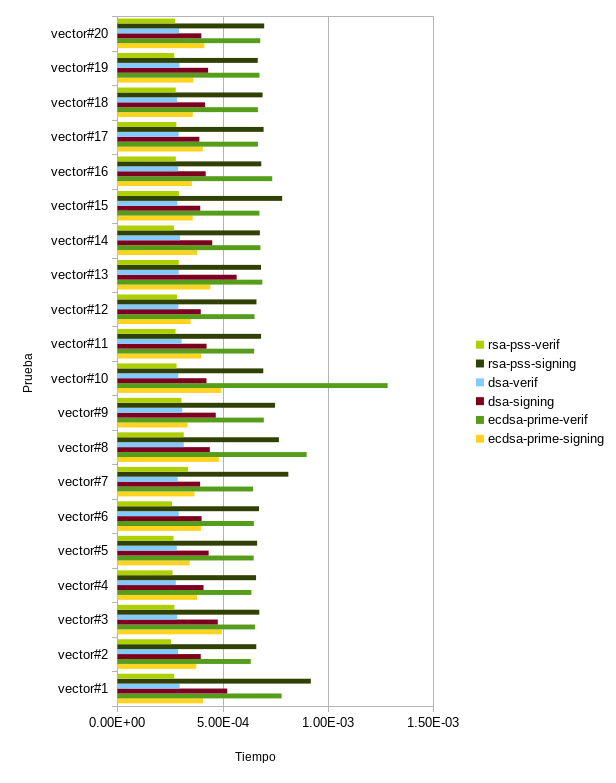
\includegraphics[width=\textwidth]{rsa_sign_verif_res}
  \caption{Resultado Firma y verificación}\label{fig:fyv}
\end{subfigure}
\hfill{}
\begin{subfigure}[b]{0.45\textwidth}
  \centering
  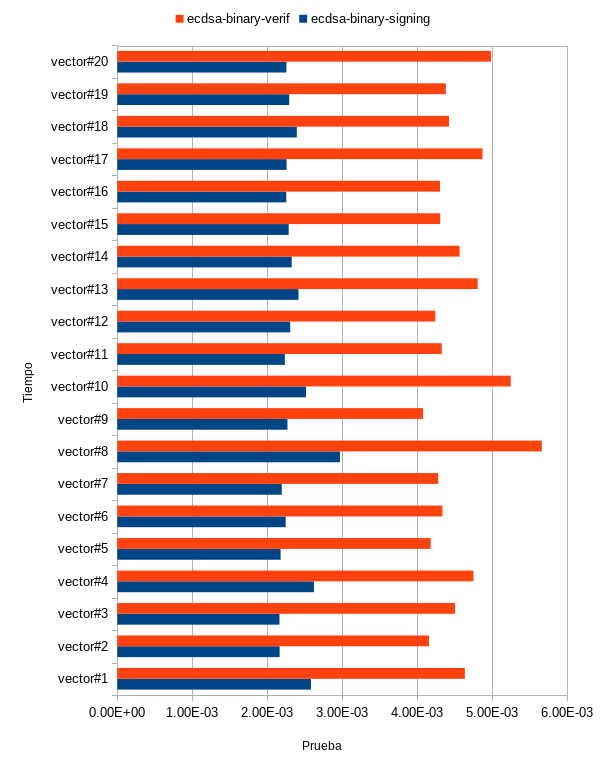
\includegraphics[width=\textwidth]{rsa_sign_verif-bin_res}
  \caption{Resultado Firma y verificación (binario)}\label{fig:fyvbin}
\end{subfigure}
\caption{Gráficas de firma y verificación}\label{fig:fv}
\end{figure}

A medida que aumenta el nivel de seguridad requerido, la ventaja se inclina aún más
radicalmente hacia \textit{ECDSA}, eso se debe a que debe aumentar el tamaño del módulo
\textit{RSA} mucho más rápido que el tamaño de la curva \textit{ECDSA} para aumentar el
nivel de seguridad.



\end{document}
